\documentclass[pdftex,letterpaper,12pt]{report}
\usepackage{thesis}
\usepackage{amsmath}
\usepackage{amssymb}
\usepackage{amsthm}
\usepackage{mathtools}
\usepackage{bm}
\usepackage{gensymb}
\usepackage{wasysym}
\usepackage{mathtools}
\usepackage{physics}
\usepackage{empheq}
\usepackage{cases}
\usepackage{rotating}
\usepackage{subfig}
\usepackage{caption}
\captionsetup{labelfont=bf} 
\captionsetup[subfloat]{position=top,singlelinecheck=off,justification=raggedright,font=bf,labelfont=large,labelformat=simple,captionskip=-2mm}
\usepackage{float}
\usepackage{enumitem} 
\usepackage[toc,page]{appendix}






\begin{document}
	
\begin{equation}
\begin{split}
\nu_{m_{F}\rightarrow m_{F-1}}=&-\frac{g_{I}\mu_{N}B}{h}\\
&+\frac{h\Delta\nu_{hfs}}{2}\left(\frac{2x}{2I+1}-\frac{2(2m_{F}-1)x^{2}}{(2I+1)^{2}}+\frac{(-(2I+1)^{2}+4-12m_{F}+12m_{F}^{2})x^{3}}{(2I+1)^{3}}\right+\cdots)
\end{split}
\end{equation}

\section{section}
\subsection{sub}
\subsubsection{sub1}
\subsubsection{sub2}

\begin{figure}[H]
	\centering
	\resizebox{0.91\textwidth}{!}{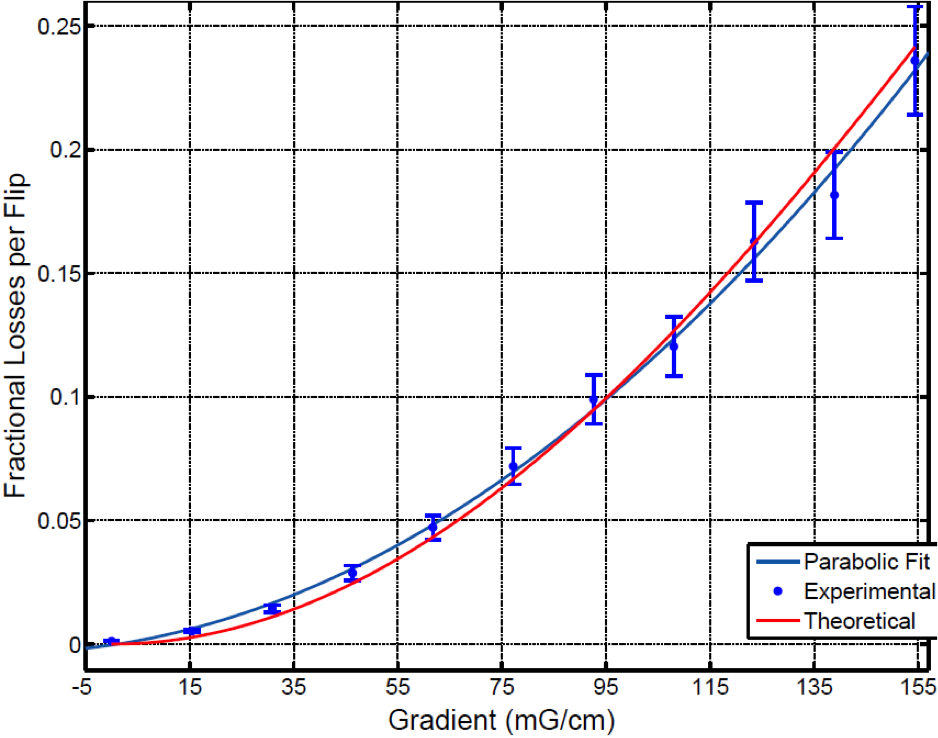
\includegraphics{AFPLossvsGradient.png}}
	\caption{{\bf Fractional AFP loss (single flip) as a function of field gradient.}}
	\label{AFPLossvsGradient}
\end{figure}

\emph{et al.}
5P$_{\frac{3}{2}}\rightarrow$

\addcontentsline{toc}{chapter}{Bibliography}
\bibliography{ref}

\end{document}